\input{Packages}
\input{Definitions}
\DeclareRobustCommand{\stirling}{\genfrac\{\}{0pt}{}}
%this removes numbering from the section, from some reason the \section*{} command doesnt work once you redefine it
\setcounter{secnumdepth}{0} 

% Define variables for week number and meeting date
\newcommand{\weekNum}{6} % Change this to update the week number
\newcommand{\meetingDate}{February 26th, 2025} 

\begin{document}
\pagestyle{empty}
\sloppy
\maketitle
 
\section{Topic: Divisibility}

\begin{problem}[D][1][AMATYC Fall 2007/13]
    % Divisibility ^ Primes ^ Student Math League
    Add any integer \( N \) to the square of \( 2N \) to produce an integer \( M \). For how many values of \( N \) is \( M \) prime?
\end{problem}\vspace{5pt}
\hspace{10pt}A. 0\hfill B. 1\hfill C. 2\hfill D. A finite number \(> 2\)\hfill E. An infinite number\hspace{10pt}

\begin{solution}[C]
    We have
    \(
        M = (2N)^2+N = 4N^2+N = N(4N+1).
    \)
    Since we can write \(M\) as a product of two numbers, it will almost never be prime. For \(M\) to be prime, one factor must be \(\pm1\) and the other would need to be prime. We'll consider this case by case.
    
    If \(4N+1 = 1\) we get \(N=0\), giving \(M=0\) which is not prime, and if \(4N+1 = -1\) we get \(N=\frac{1}{2}\) which is clearly not an integer. So neither of these cases work.
    
    If \(N=1\) then \(M=5\) and if \(N=-1\) then \(M=3\), so both of these cases work. Thus we have \fbox{2} solutions.
\end{solution}

\begin{problem}[D][2][MONT 1.12/1]
    % Divisibility ^ Primes ^ MONT
    Show that any composite number \(n\) has a prime factor \(\leq \sqrt{n}\).
\end{problem}

\begin{solution}
    A composite number is a integer with at least 2 prime factors. Consider a prime factor \(p\) of \(n\), and suppose \(p>\sqrt{n}\). Then there is some integer factor \(k\) such that \(pk=n\), and so we have
    \[
        pk > k\sqrt{n} \quad \Rightarrow \quad n>k\sqrt{n} \quad \Rightarrow \quad \sqrt{n}>k
    \]
    Since \(k\) is either prime or a product of primes, and we now know \(k<\sqrt{n}\), there must be at least one prime \(q<\sqrt{n}\) such that \(q \mid k\). And since \(k \mid n\), we have \(q \mid n\). So \(q\) is a factor of \(n\) and therefore \(n\) has at least one prime factor \(\leq \sqrt{n}\). $\Box$
\end{solution}

\begin{problem}[D][3][AMATYC Fall 2018/1]
    % Divisibility ^ Pigeonhole Principle ^ Student Math League
    Let M be the greatest integer less than 30 such that \(M!(M+1)!/2\) is a perfect square. Let N be the greatest integer that divides \(c^4 - c^2\) for all integers \(c > 1\). Find \(M + N\).
\end{problem}
\multOpt[5]{19}[21][26][29][36]

\begin{solution}[D]
    To find \(M\), recall that \((k+1)!=(k+1)k!\). Using this property, we find that
    \[
        \frac{M!(M+1)!}{2} = \frac{(M+1)(M!)^2}{2} = \frac{M+1}{2}(M!)^2
    \]
    So we need \(\frac{M+1}{2}\) to be a perfect square. Thus, the largest \(M<30\) we can choose is \(M=17\) so that \(\frac{M+1}{2} = 9\).

    To find \(N\), observe that \(c^4-c^2 = c^2(c^2-1) = c^2(c-1)(c+1)\). Importantly, here we have the product of three consecutive numbers, the middle of which is repeated. Grouping \((c-1)(c)\) and \((c)(c+1)\), we can see that both are divisible by 2, since at least one factor of each is even. Also, grouping \((c-1)(c)(c+1)\), we can see one of these will be divisible by 3. (In general, the product of \(k\) consecutive terms will be divisible by \(k\).) Thus, the largest integer which divides \(c^4-c^2\) is \(N=2\cdot2\cdot3=12\).

    Finally, then, we have \(M+N = 17+12=\boxed{29}\).
    \end{solution}

\begin{problem}[D][2][Folklore]
    % GCD ^ Fibonacci 
    Let $F$ be the Fibonacci Sequence, defined as $F_1=F_2 = 1$ and $F_n = F_{n-1} + F_{n-2}$ for $n \geq 3$. Show that all pairs of consecutive Fibonacci numbers are relatively prime. (that is, their GCD is 1).
\end{problem}

\begin{solution}
    This one is quite simple if you are familiar with the property \(\gcd(a,b)=g(a+b,b)\). First, note that for \(F_1=1\) and \(F_2=1\), clearly \(\gcd(F_1,F_2)=1\). This serves as our base case. Next, observe that if we have \(\gcd(F_{n}, F_{n+1})=1\), then
    \[
        \gcd(F_n,F_{n+1})= \gcd(F_n+F_{n+1}, F_{n+1}) = \gcd(F_{n+2}, F_{n+1}).
    \]
    So if a pair of consecutive Fibonacci numbers are coprime, the next pair is also coprime. Thus, by induction, all pairs of consecutive Fibonacci numbers are relatively prime. $\Box$
\end{solution}

\begin{problem}[D][3][2006 AMC 12A/14]
    % Bezout's Identity ^ AMC
    Two farmers agree that pigs are worth $300$ dollars and that goats are worth $210$ dollars. When one farmer owes the other money, he pays the debt in pigs or goats, with "change" received in the form of goats or pigs as necessary. (For example, a $390$ dollar debt could be paid with two pigs, with one goat received in change.) What is the amount of the smallest positive debt that can be resolved in this way?
\end{problem}
\multOpt[5]{5}[10][30][90][210]

\begin{problem}[D][4][AMATYC Fall 2020/16]
    % Divisibility ^ Primes ^ Student Math League
    Let M be the unique whole number less than 200 that has exactly 18 whole number factors. Find the sum of all 18 factors of M.
\end{problem}
\multOpt[5]{$545$}[$546$][$601$][$602$][$646$]

\begin{problem}[D][6][AMATYC Spring 2016/11]
    % Divisibility ^ Simon's Favorite Factoring Trick ^ Student Math League
    Every integer $N > 0$ can be represented in at least one way as $ab - (a + b)$, where $a$ and $b$ are positive integers with $a \leq b$. Find the smallest $N$ having at least 3 such representations.
\end{problem}

\begin{problem}[D][3][All Russia Mathematics Olympiad 1995]
    % Divisibility ^ GCD
    Let \( m, n \) be positive integers such that
    \[
    \gcd(m, n) + \operatorname{lcm}(m, n) = m + n.
    \]
    Show that one of the two numbers is divisible by the other.
\end{problem}

\begin{problem}[D][6][Russia 1995 10/5]
     % Divisibility ^ GCD
    Let $a_1, a_2, \ldots, $ be an infinite sequence such that for any integers $i,j \in \mathbb{Z}^+$ we have $\gcd(a_i, a_j) = \gcd(i, j)$. Show that $a_n = n$ for any $n \in \mathbb{Z^+}$.
\end{problem}


\begin{problem}[D][4][Cuba 2022/2]
     % Divisibility 
    We say that a positive integer $n$ is alternative if the following property is true: For each divisor $d$ of $n$, we have that $d+1$ is a divisor of $n+1$. Find all the alternative positive integers.
\end{problem}

\begin{problem}[D][6][Andreescu]
     % Divisibility ^ GCD
    Find all pairs of positive integers $(a,b)$ such that 
    \begin{align*}
        \frac{ab}{a + b} \in \mathbb{Z}.
    \end{align*}
\end{problem}

\begin{problem}[D][5][Spain 2015/5]
     % Divisibility ^ GCD ^ MOD
    Let $p$ and $n$ be integers, such that $p$ is prime, $n \geq p$, and $1 + np$ is a perfect square. Show that $n + 1$ is the sum of $p$ nonzero perfect squares.  
\end{problem}

\section{Other Fun Stuff}\setcounter{problem}{0}

\begin{problem}[F][4][BMT 2024 Geometry/3]
     % Geometry ^ BMT
    A square with side length 6 has a circle with radius 2 inside of it, with the centers of the square and circle vertically aligned. Aarush is standing 4 units directly above the center of the circle, at point P. What is the area of the region inside the square that he can see?

    \begin{center}
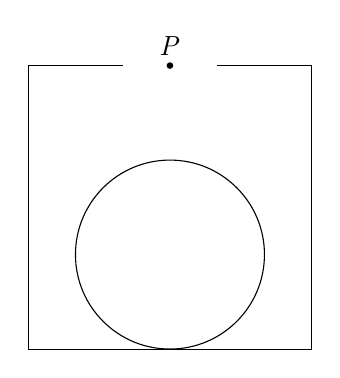
\begin{tikzpicture}[scale = 0.6]
    % Define center of square and circle
    \coordinate (O) at (0,0);
    
    % Draw square
    \draw (-3,-3) rectangle (3,3);
    \fill[white] (-1,2.8) rectangle (1,3.2);
    
    % Draw circle
    \draw (0, -1) circle (2);
    
    % Define and draw point P
    \coordinate (P) at (0,3);
    \fill (P) circle (2pt);
    \node[above] at (P) {\textit{P}};
\end{tikzpicture}
\end{center}
\end{problem}

\begin{problem}[F][4][BMT 2024 Discrete/4]
     % Divisibility ^ BMT
    Eight players are seated around a circular table. Each player is assigned to either Team Green or Team Yellow so that each team has at least one player. In how many ways can the players be assigned to the teams such that each player is on the same team as at least one player adjacent to them?
\end{problem}

\begin{problem}[F][3][2025 AIME II/4]
   %AIME ^ Telescopic Cancellation
The product
\begin{align*}
\prod_{k=4}^{63} \frac{\log_k(5^{k^2-1})}{\log_{k+1}(5^{k^2-4})} = \frac{\log_4(5^{15})}{\log_5(5^{12})} \cdot \frac{\log_5(5^{24})}{\log_6(5^{21})} \cdot \frac{\log_6(5^{35})}{\log_7(5^{32})} \cdots \frac{\log_{63}(5^{3968})}{\log_{64}(5^{3965})}
\end{align*}
is equal to $\frac{m}{n}$, where $m$ and $n$ are relatively prime positive integers. Find $m + n$.
\end{problem}

\begin{problem}[F][2]
   % Discrete ^ Knights and Knaves
On an island, the inhabitants are either knights, who always tell the truth, or knaves, who always lie. One day, three of these inhabitants—A, B, and C—were standing together in a garden when a stranger passed by. The stranger asked A, "Are you a knight or a knave?" A answered, but rather quietly, so the stranger could not make out what he said. The stranger then turned to B and asked, "What did A say?" B replied, "A said that he is a knave." At this point, the third man, C, spoke up. "Don't believe B; he is lying!"\\

    What are B and C?
\end{problem}




\end{document}